%!TEX root =  A_WS.tex

\section*{Practice Exam 1B}  
\markright{Practice Exam 1B}
\addcontentsline{toc}{section}{Practice Exam 1B}

\emph{Try taking this version of the practice exam under testing conditions:  no book, no notes, no classmate's help, no electronics (computer, cell phone, television). Give yourself one hour to work and wait until you have tried your best on all of the problems before checking any answers.}

\noindent \hrulefill

\begin{enumerate}

\item The amount of money spent on nursing home care for seniors has continued to rise.  The table shows the values for select years.  Here $S$ is the spending, measured in billions of dollars and $Y$ is the year, measured in years since 1960.

\begin{center}
\begin{tabular} {|c ||c |c |c |c |c |c |c |} \hline
$Y$ & 0 & 10 & 25 & 40 & 52 \\ \hline
$S$ & 1.0 & 3.3 & 33.7 & 96.6 & 170.3 \\ \hline
\end{tabular}
\end{center}

\begin{enumerate}
\item According to the table, what was the spending in 1970?  \vfill
\item According to the table, what was the spending in 1985?  \vfill
\item Calculate the rate of change of spending over the period 1970 to 1985.  Don't forget to state the units. \vfill \vfill
\item In approximately what year did spending first pass \$50 billion? \vfill
\end{enumerate}

\newpage

\item Trish is filling a swimming pool with water.  The graph below shows how many gallons of water ($G$) are in the pool after $H$ hours.  Use the graph to answer the following questions.
\begin{center}
\scalebox {.9} {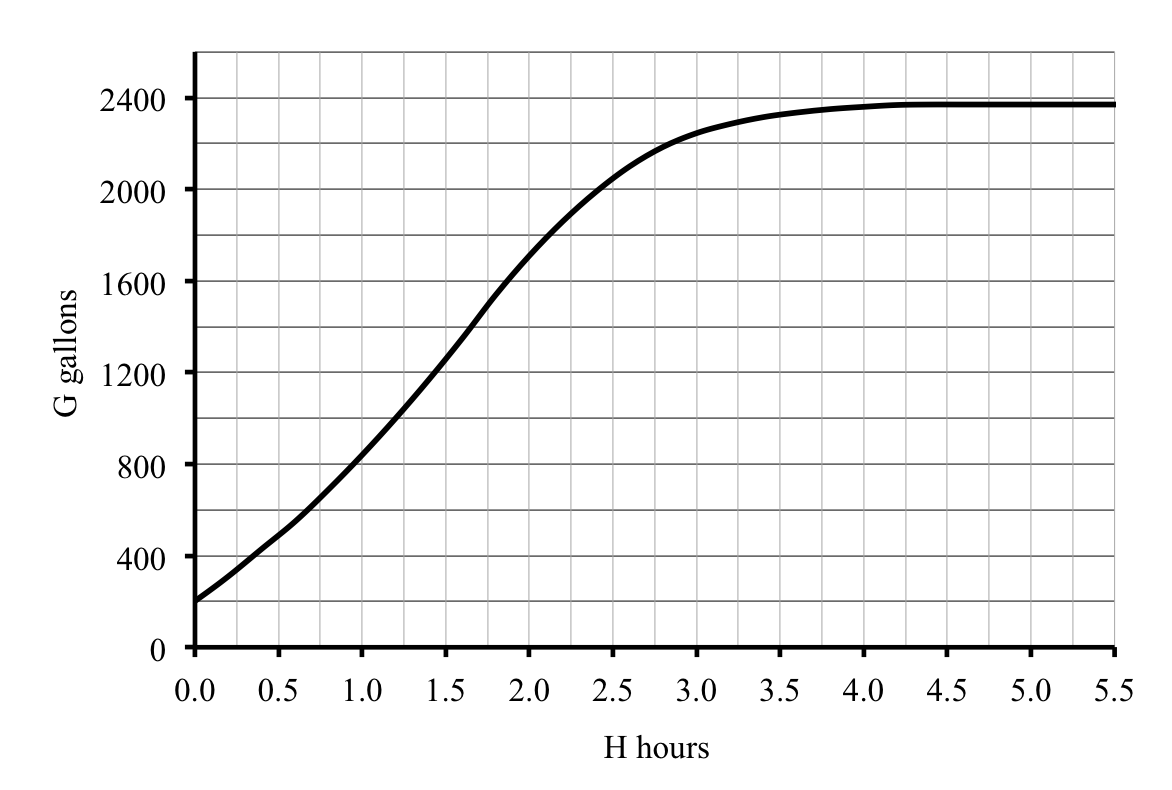
\includegraphics [width = 6in] {fillingtankNEW}}
\end{center} 
\begin{enumerate}
\item How much water was in the swimming pool already when Trish began? \vfill
\item How much water was in the swimming pool after 3 hours? \vfill
\item After how many hours were there \text{1,000} gallons of water in the swimming pool? \vfill
\item Was Trish filling the pool faster at 2 hours or at 2.5 hours?  Explain how you see that on the graph. \vfill
\item After (about) how many hours did Trish stop filling the swimming pool?  Explain how you see that on the graph. \vfill
\end{enumerate}

\newpage

\item In 1990 the Lef\`evre's property tax was \$450 but it doubled every year thereafter.  
 \begin{enumerate}
 \item Name the variables, including units. \vfill \vfill
 \item Which is the independent variable and which is the dependent variable? \vfill
\item Make a table showing the property tax each year from 1990 to 1994. \vfill \vfill
\item Draw a graph illustrating the dependence.
\bigskip
\begin{center}  
\scalebox {.8} {
\includegraphics [width = 6in] {GraphPaper.jpg}}
\end{center}
\bigskip
 \end{enumerate} 
 
\newpage

\item The distance from the Earth to the Moon is approximately \text{384,000,000} meters. 

\hfill \begin{footnotesize} Source:  Wikipedia (Lunar distance)\end{footnotesize}
\begin{enumerate}
\item Express this distance in scientific notation. \vfill
\item Express this distance in kilometers (km), using $1 \text{ km} = \text{1,000 meters}$. \vfill \vfill
\item Express this distance in miles, using the conversion $1 \text{ mile} \approx 1.609 \text{ km}$. \vfill \vfill
\item If you could drive to the moon at 55 mph, how long would it take to get there? Express your answer in terms of months, using $1 \text{ month} \approx 30 \text{ days}$. \vfill \vfill \vfill
\end{enumerate}

%%%% END

\end{enumerate}

